\documentclass[conference]{IEEEtran}
\usepackage[utf8]{inputenc}

\usepackage[portuguese]{babel}

\usepackage{multirow}

\usepackage{datetime}

\usepackage[table,xcdraw]{xcolor}

\usepackage[pdftex]{graphicx}
\graphicspath{{./Imagens/}}

\usepackage{adjustbox}

% correct bad hyphenation here
\hyphenation{op-tical net-works semi-conduc-tor DEFCON}

\begin{document}

%
%
% ------------------------------------------------------------

\title{How private is my medical information?\\
	\vspace*{10pt} \large Sociologia e Ética da Informática\\
		\normalsize \today{} }
%
\author{Vanessa Silva\\
	{\texttt{(up201305731@fc.up.pt)}}\\
	\multicolumn{1}{p{.7\textwidth}}{\centering\emph{
		\\Departamento de Ciências de Computadores,\\Faculdade de Ciências da Universidade do Porto}}
}

\maketitle

% ------------------------------------------------------------

%----------------------ABSTRACT----------------------%

\begin{abstract}

% deve indicar de forma clara o que vai tratar o relatório (5-6 linhas).

\end{abstract}


% ------------------------------------------------------------

\IEEEpeerreviewmaketitle

%----------------------INTRODUÇÃO----------------------%

\section{Introdução}

% introduzir o tema de forma clara (o que é, em que consiste, quando e como surgiu, para que serve, ...), fazer o enquadramento (semelhanças e/ou diferenças) com os restantes tópicos apresentados nas aulas e descrever sumariamente a organização do relatório.

\section{Secção sobre conceitos/terminologia e entidades de saúde}

% organizar segundo o tema em questão e segundo os tópicos que pretende realçar. Uma das secções pode ser usada para referenciar ou comparar trabalhos relacionados.

\subsection{Terminologia}

\begin{itemize}

	\item \textbf{Dados pessoais} - qualquer informação, independentemente da natureza e do respetivo suporte, incluindo som e imagem, relativa a uma pessoa singular identificada ou identificável (titular dos dados); sendo que uma pessoa é considerada identificável pode ser identificada direta ou indiretamente, por referência a um número de identificação ou a um ou mais elementos específicos da sua identidade física, fisiológica, psíquica, económica, cultural ou social \cite{parecerERS2015}, \cite{CNPDinfsaude2014}.
	
	\item \textbf{Informação médica} - informação de saúde destinada a ser utilizada em prestações de cuidados ou tratamentos de saúde \cite{regulamentodeonmedic}.
	
	\item \textbf{Informação de saúde} - qualquer informação direta ou indiretamente ligada à saúde, presente ou futura, de uma pessoa, quer se encontre com vida ou tenha falecido, e a sua história clínica e familiar \cite{consolidacaoinfsaude}.
	
	\item \textbf{Processo clínico} - qualquer registo, informatizado ou não, que contenha informação de saúde sobre doentes ou sobre os seus familiares. Deve conter toda a informação médica disponível que diga respeito ao doente, incluindo a sua situação atual, evolução futura e história clínica e familiar, bem como de informação suficiente sobre a identificação do doente \cite{regulamentodeonmedic}, \cite{parecerERS2015}. 
	
	\item \textbf{Ficha clínica} - é o registo dos dados clínicos do doente e das anotações pessoais do médico. Tem como finalidade a memória futura e a comunicação entre os profissionais que tratem o doente \cite{regulamentodeonmedic}.
	
	\item \textbf{Processo clínico eletrónico} - agrega informação médica dispersa de um doente, pode conter dados relativos à sua história clínica, exames físicos e complementares, diagnósticos, intervenções cirúrgicas, e são introduzidos e visualizados de forma estruturada. Permite a articulação entre vários serviços de saúde, a consulta e o pedido em \textit{real time} de meios complementares de diagnóstico, bem como a partilha da informação entre o utente, os profissionais de saúde e as instituições \cite{CNPDinfsaude2014}.
	
	\item \textbf{Tratamento de dados pessoais} - qualquer operação ou conjunto de operações efetuadas sobre os dados pessoais, com ou sem meios automatizados, tais como recolha, registo, organização, conservação, adaptação ou alteração, recuperação, consulta, utilização, comunicação, bloqueio, eliminação ou destruição \cite{parecerERS2015}.
	
	\item \textbf{Dados anonimizados} - alteração do processo clínico impossibilita a vinculação dos doentes com os seus dados \cite{safran2007toward}.
	
	\item \textbf{Dados de-identificados} - eliminação de todos os identificadores, ou seja, nome do doente, número de utente, número de segurança social, e outros dados que vinculam diretamente um doente com os seus dados \cite{safran2007toward}.
	
	\item \textbf{Dados anonimizados reversíveis} - alteração do processo clínico de forma a que a re-identificação possa ser realizada através do acesso a uma chave protegida que permita vincular os doentes com os seus dados \cite{safran2007toward}.
	
	\item \textbf{Privacidade} - direito fundamental de cada indivíduo de decidir quem deve ter acesso aos seus dados pessoais \cite{segurancaSI}.
	
	\item \textbf{Confidencialidade} - disponibilidade de medidas e mecanismos para manter a privacidade do doente, e proporcionando uma estrutura que permita dar acesso a informação privada, a quem foi dada autorização para tal \cite{segurancaSI}.
	
\end{itemize}

\subsection{Entidades controladoras do sistema de saúde}

\begin{itemize}

	\item \textbf{Comissão Nacional de Proteção de Dados (CNPD)}: Entidade administrativa independente, com poderes de autoridade, que funciona junto da Assembleia da República. Tem como função controlar e fiscalizar o cumprimento das disposições legais na matéria de proteção de dados pessoais, em rigoroso respeito pelos direitos do homem e pelas liberdades e garantias consagradas na Constituição e na lei.
	
	\item \textbf{Ordem dos Médicos}: Associação pública que representa os médicos que exercem a profissão em Portugal, distribuídos por especialidades, sub-especialidades e competência, cuja principal missão é promover a defesa da qualidade dos cuidados de saúde prestados à população, bem como o desenvolvimento, a regulamentação e o controlo do exercício da profissão de médico, assegurando a observância das regras de ética e deontologia profissional.
	
	\item \textbf{Gabinete Nacional de Segurança/Centro Nacional de Cibersegurança (GNS/CNCS)}: Tem como principal objetivo contribuir para que o país use o ciberespaço de forma livre, mas, e acima de tudo, de forma confiável e segura, através da promoção de uma contínua melhoria da cibersegurança nacional e da cooperação internacional, bem como da implementação de medidas e instrumentos necessários para antecipar, detetar, reagir e recuperar de situações que, face à ocorrência de incidentes ou ciberataques, ponham em causa o funcionamento das infraestruturas críticas e os interesses nacionais \cite{colabCNCS_SPMS}.
	
	\item \textbf{Serviços Partilhados do Ministério da Saúde (SPMS)}: Tem com principal objetivo a cooperação, a partilha de conhecimento e informação e o desenvolvimento de atividades de prestação de serviços nas áreas dos sistemas e tecnologias de informação e de comunicação, garantindo a operacionalidade e segurança das infraestruturas tecnológicas e dos sistemas de informação do Ministério da Saúde.

\end{itemize}

Dados as competências particulares e objetivos comuns, no passado dia 21 de fevereiro de 2017, o SPMS assinou com o GNS/CNCS um protocolo de cooperação. Este protocolo visa promover a otimização de procedimentos e uma maior eficiência no sistema, estabelecendo as formas de cooperação entre as partes no desenvolvimento das capacidades nacionais de cibersegurança, troca de conhecimento e aprofundamento das capacidades.


\section{Secção do Desenvolvimento}

\subsection{Motivação}

A recolha da informação médica é feita durante uma consulta médica, essencialmente através da narrativa do doente, de exames complementares e através da consulta ao processo e à ficha clínica anterior do doente, caso exista.

A informação que consta num processo clínico corresponde a informação maioritariamente alfanumérica, ou seja, que pode ser representada por carateres ou dígitos. Enquanto que a restante informação, proveniente dos meios complementares de diagnóstico, como sinal ou imagem, normalmente não consta no processo clínico, por exemplo imagens de ressonâncias magnéticas só são visualizadas quando explicitamente solicitadas, não ficando assim toda a informação clínica de um dado doente disponível como um todo \cite{santos2010comunicaccao}.

Na verdade, muitas das vezes os profissionais de saúde não dispõem de toda a informação sobre os doentes, o que poderá refletir-se na qualidade e nos resultados da sua intervenção. Estas falhas no acesso à informação médica podem conduzir a quebras na continuidade dos serviços prestados, a tratamentos/procedimentos inadequados ou pouco eficazes, com efeitos negativos para o bem-estar do doente \cite{santos2010comunicaccao}. 

\begin{figure}[!ht]
    \centering
    \begin{minipage}{.9\textwidth}
        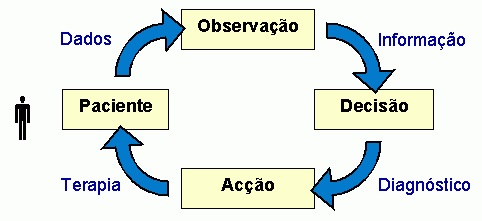
\includegraphics[width=0.53\textwidth]{diagnostico_terapeutica.png}
        \label{fig1}
    \end{minipage}%
    \caption{Ciclo clínico \cite{regclinelect}.}
\end{figure}
 
O processo clínico em papel é uma forma de registo clínico onde os dados são escritos pelo proficional de saude, e toda a informação clínica complementar é anexada a este. Este é um sistema de armazenamento, que serve de base à prestação de cuidados de saúde, e por isso, necessita de integrar informação proveniente de diversas fontes \cite{regclinelect}. Mas com o decorre dos anos este formato em papel começou a desencadear vários inconvenientes devido à diversidade da estruturação da informação, que depende do médico e/ou da instituição, ou a falta dela, ao acesso limitado à informação bem como a dificuldades na localização de determinada informação, à ilegibilidade dos registos médicos, e a perdas e duplicação de informação \cite{regclinelect}.

Com o avanço da tecnologia, surgiram os processos clínico eletrónicos que visam não só colmatar as limitações referidas, bem como fornecer uma variedade de ferramentas auxiliares que permitam ajudar na decisão clínica, avaliar a qualidade dos cuidados prestados, ajudar na investigação e na educação médica, realizar a gestão e o planeamento dos recursos de saúde, e possibilitar a troca de informação clínica entre cuidados primários e hospitalares. Mas, em contrapartida, toda esta informatização implica um elevado nível de proteção e segurança dada a sensibilidade da informação clínica e pessoal contida nos processos clínicos eletrónicos.

As preocupações de proteção e segurança derivam do facto de que as diferentes instituições podem partilhar estas informações sensíveis entre si, confiando mutuamente que a informação irá ser mantida confidencial e será apenas usada para o propósito definido, assim como nas trocas de informação entre profissionais da mesma instituição. Contudo, o resultado desta partilha pode não ser o esperado, por isso é de grande preocupação o facto de que estes profissionais podem aceder à informação médica, não só da rede da sua instituição de trabalho como também de outras instituições. Isto torna difícil a gestão e a auditoria de quem tem, ou teve, acesso e a que informação, bem como saber quais os mecanismos de segurança o sistema deve ter.

O problema da segurança nos sistemas de informação é um dos temas mais falados na atualidades não só relacionados à área da saúde como a todas as outras área. Deve-se, ainda, ter especial atenção a problemas relacionado, como a confidencialidade, uma vez que a grande acessibilidade aos dados implica uma grande ameaça para a privacidade dos doentes, devendo-se adotar medidas para prevenir a ocorrência de acessos não autorizados; como a integridade, pois erros nos dados e no \textit{software} podem acontecer, devendo-se adotar medidas de proteção contra a perda ou corrupção dos dados; e como a disponibilidade, dado que as instituições de saúde ficam cada vez mais dependentes do funcionamento dos sistemas de informação, devendo-se adotar medidas para que o acesso autorizado a informação confidencial esteja disponível sempre que necessário. Ver tabela \ref{tabl1}.

\begin{table*}[!ht]
\centering
\caption{Técnicas de prevenção e deteção/correção de problemas relacionados com a segurança \cite{segurancaSI}.}
\label{tabl1}
\begin{adjustbox}{max width=\textwidth 	}
\begin{tabular}{ |l|l|l| }

\hline
	\multicolumn{1}{|c|}{\cellcolor[HTML]{EFEFEF}{\color[HTML]{333333}}}	&	\multicolumn{1}{|c|}{\cellcolor[HTML]{EFEFEF}{\color[HTML]{333333} \textbf{Prevenção}}}	&	\multicolumn{1}{|c|}{\cellcolor[HTML]{EFEFEF}{\color[HTML]{333333} \textbf{Deteção/Correção}}}	\\
\hline

\multirow{3}{*}{\textbf{Confidencialidade}}			&	controlar acesso					&	auditoria					\\
													&	autenticação						&	monitorização				\\
													&	encriptação							&								\\
\hline

\multirow{4}{*}{\textbf{Confidencialidade}}			&	assinaturas digitais				&	assinaturas digitais		\\
													&	apoio à introdução de dados			&	auditoria					\\
													&	\textit{standards} e codificações	&	monitorização				\\
													&	métodos de consistências interna	&								\\
\hline

\multirow{4}{*}{\textbf{Disponibilidade}}			&	redundância de equipamento			&	redundância de equipamento	\\
													&	sistemas de recuperação automática	&	auditoria					\\
													&										&	monitorização				\\
													&										&	backups 					\\
\hline

\end{tabular}
\end{adjustbox}
\end{table*}

Rapidamente se percebe que para uma melhor proteção da informação deve-se aplicar as medidas de segurança tanto a nível dos equipamentos e do \textit{software}, como das pessoas e dos procedimentos. Garantir uma segurança perfeita é ainda impossível, no entanto é possível reduzir os riscos ou restringir possíveis danos devido à má utilização e/ou ao uso abusivo dos sistemas de informação.


\subsection{Princípios éticos}

Todas as instituições estão sujeitas a princípios éticos, e como tal as ações dos profissionais de saúde estão sujeitas a esses princípios, o qual se destaca o sigilo médico. Adicionalmente, quando estes princípios se aplicam no âmbito da informática, destaca-se desde logo o princípio da privacidade e o princípio da segurança, uma vez que todos os doentes têm o direito à privacidade e ao controlo da recolha, do armazenamento, do acesso, do uso e da transmissão da sua informação médica, e os dados recolhidos pelos profissionais de saúde devem ser protegidos contra a perda, corrupção, destruição, acesso, uso e alteração indevida ou não autorizada \cite{segurancaSI}.

Perante toda a disponibilidade de informação clínica aos profissionais de saúde, que por um lado é essencial para uma melhor prestação de serviços mas que por outro pode ser em demasia e põe em causa questões muito sérias sobre a segurança dos dados. Inclusive, recentemente, o Bastonário da Ordem dos Médicos, Miguel Guimarães, afirmou o seguinte, "Os médicos têm potencialmente acesso a qualquer informação clínica de um doente e nem sei se deviam ter acesso a todas. Mas não são só os médicos que têm acesso, há outros profissionais que também têm", e, em defesa dos médicos, afirma que, "Isto é um problema atual. Mas quem é responsável pela partilha dessa informação de doentes não são os médicos", uma vez que, "Numa questão em que os dados passam a estar disponíveis num local em que potencialmente podem ter vários utilizadores, tenho dúvidas que a responsabilidade dessa partilha deva ser do médico e não do Estado português".

Com vista a melhorar a proteção de dados relacionados à saúde, uma série de leis e regulamentos foram propostos e atualizados nos últimos anos.

Segundo o Regulamento de Deontologia Médica n.º707/2016, de 21 de Julho, "O Código Deontológico da Ordem dos Médicos é um conjunto de normas de comportamento que serve de orientação nos diferentes aspetos das relações humanas que se estabelecem no decurso do exercício profissional da medicina.". Diante destas normas, está bem explícita a obrigatoriedade do segredo médico, quer singular ou coletivamente, em unidades de saúde públicas, sociais, cooperativas ou privadas, no que diz respeito às informações que constem do processo individual do doente. É ainda dever das unidades de saúde e dos diretores clínicos impedir o acesso indevido de terceiros aos processos clínicos e aos sistemas informáticos que contenham informação de saúde.
Consoante o artigo 32.º, o dever de segredo médico deixa de ser aplicado apenas e só mediante o consentimento do doente (ou representante legal), se a revelação não prejudicar terceiros com interesse na manutenção do segredo, e não pode ser revelado mais do que o extremamente necessário. O mesmo é válido para as informações que revelem um nascimento ou um óbito, e de doenças de declaração obrigatória.

Perante ainda o artigo 36.º do regulamento, sobre dados médicos informados, todos os ficheiros, bases e bancos de dados com informações clínicas sujeitas a segredo médico, devem ser equipados com sistemas, e utilizados com procedimentos de segurança, que impeçam a consulta, alteração e destruição de dados por pessoas não autorizadas, e que detetem desvios de informação, caso estas conduções não se verifiquem, os equipamentos não devem estar conectados com outros tipos de redes informáticas.


%----------------------CONCLUSÃO----------------------%

\section{Conclusões}

% resumir o que foi apresentado e indicar possíveis tópicos de continuação ou perspectivas de futuro/sucesso (10-15 linhas).

\bibliography{ref}
\bibliographystyle{IEEEtran}

\end{document}
